\documentclass{beamer}
\title{MRI Simulator Notes}
\author{Liam}
\date{\today}

\begin{document}

\begin{frame}
\maketitle
\end{frame}

\begin{frame}{Tasks}
\begin{itemize}
\item I began writing the simulation code in Python.
\item I wrote the basics of the classes Em, Pulse, and Sim.
\begin{itemize}
\item A Em object is the basic particle of simulation. Each Em has a magnetization, position, and velocity.
\item A Pulse object is a set of RF and/or gradient waveforms. A Pulse object can be in one of two modes: ``free" (x and y gradients specified) or ``excite" (RF and z gradient specified).
\item Sim is the object that runs the main simulation. Sim instantiates a number of Em objects and reads in the pulse sequence as a list of Pulse objects.
\end{itemize}
\item I tested these classes.
\begin{itemize}
\item I set $T_1 = 1$, $T_2 = 1$, $\gamma = 1$.
\end{itemize}
\end{itemize}
\end{frame}

\begin{frame}{Free precession of an em with $B_z = 10$}
\begin{center}
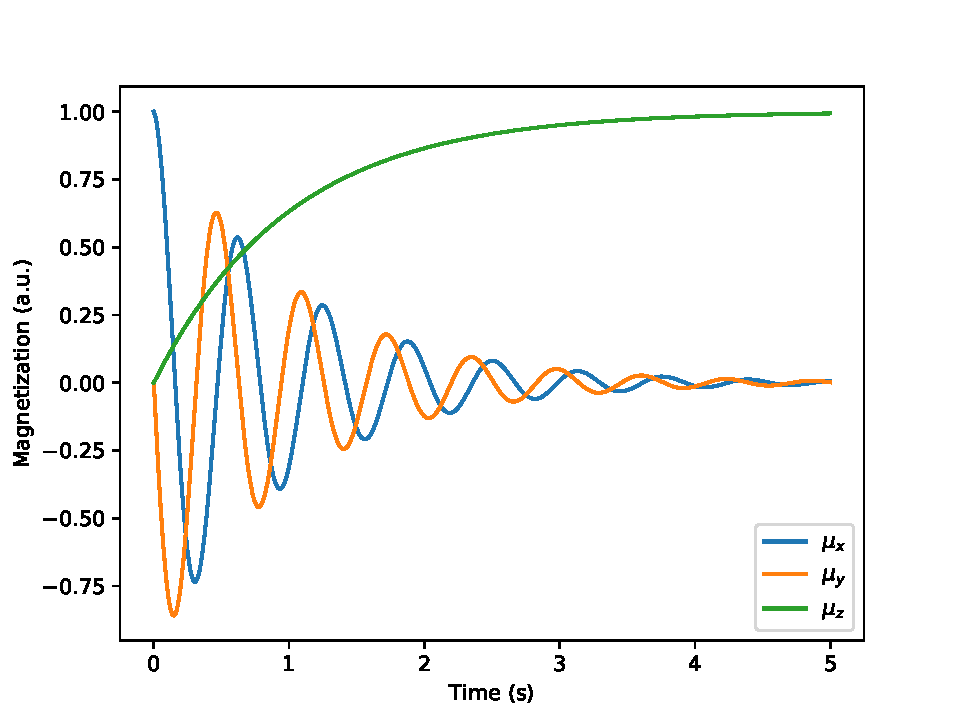
\includegraphics[height=0.8\textheight]{free_precession_em_one}
\end{center}
\end{frame}

\begin{frame}{Free precession of an em with $B_z = 20$}
\begin{center}
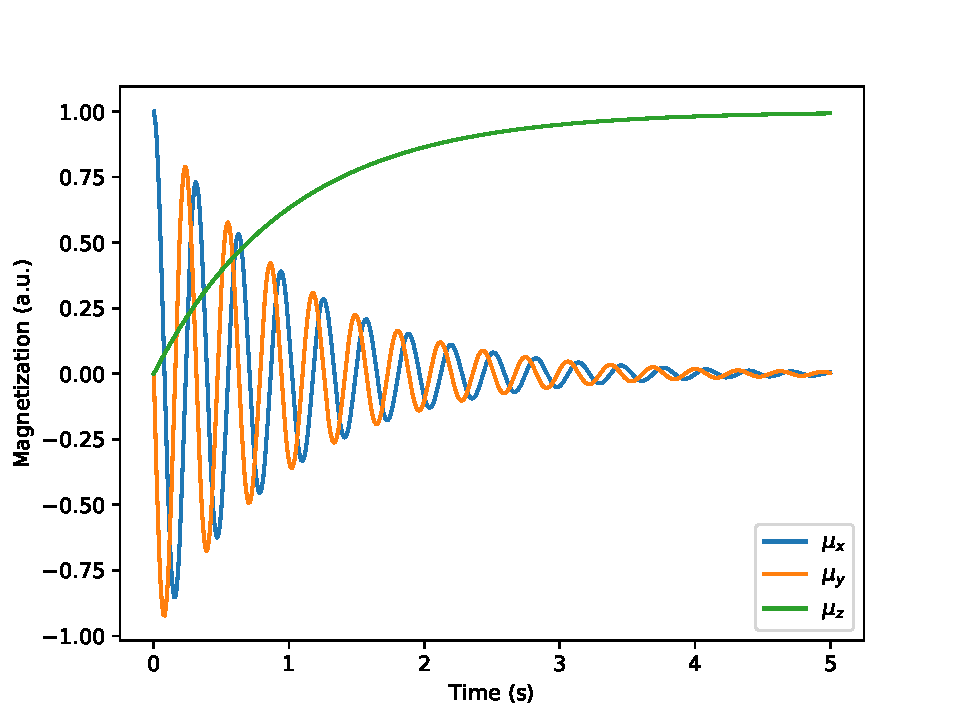
\includegraphics[height=0.8\textheight]{free_precession_em_two}
\end{center}
\end{frame}

\begin{frame}{FID of one em}
$B_0 = 10$, $G_x = 10$, em is at origin $\Rightarrow$ em experiences $B_z = 10$.
\begin{center}
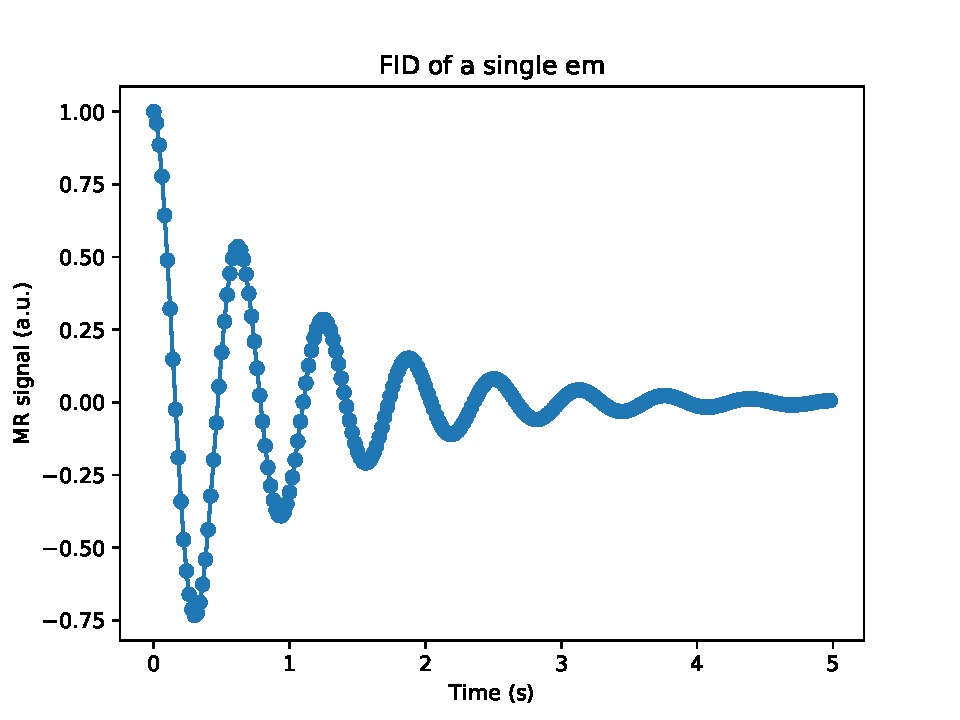
\includegraphics[height=0.8\textheight]{fid_one_em}
\end{center}
\end{frame}

\begin{frame}{FID of two ems}
$B_0 = 10$, $G_x = 10$, em one is at origin $\Rightarrow$ experiences $B_z = 10$, em two is at $x = 1$ $\Rightarrow$ experiences $B_z = 20$.
\begin{center}
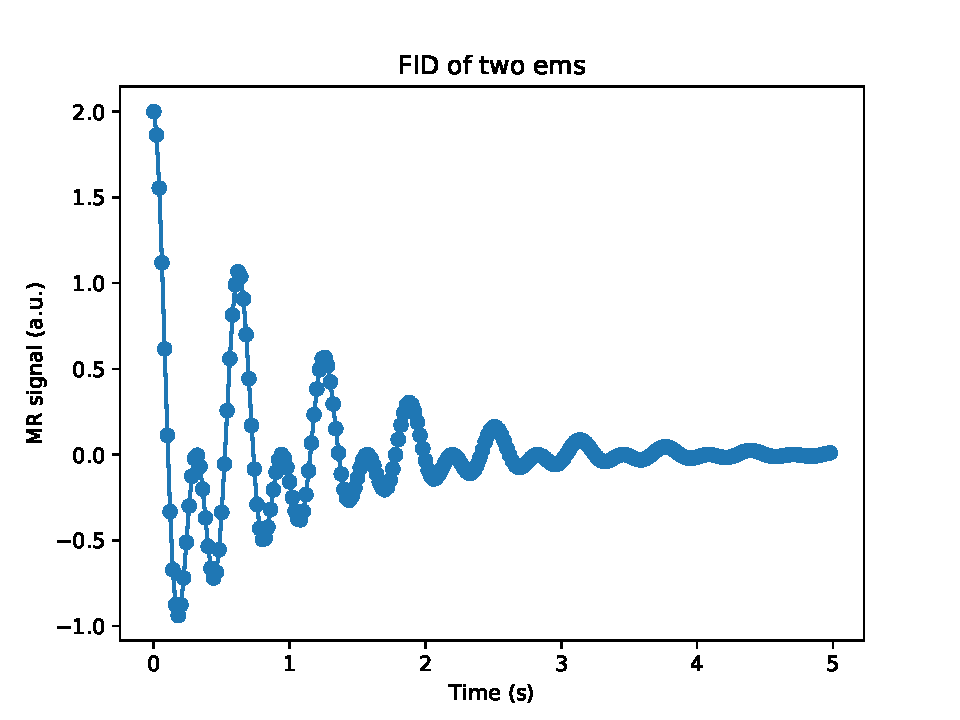
\includegraphics[height=0.8\textheight]{fid_two_ems}
\end{center}
\end{frame}

\end{document}